\chapter{Istoria conferințelor video}
\label{sec:ch2}

\section{Era analogică}
\label{sec:ch2sec1}

\indent \par Primele concepte ale transmiterii de imagini datează încă din secolul XIX, contemporane cu brevetarea telefonului de către Alexander Graham Bell în data de 14 februarie 1876 și prezentarea acestuia la Expoziția Centenară de la Philadelphia în același an. Un articol publicat în 30 martie 1877 de către The New York Sun menționează termenul \textit{electroscop} în acest context, prin care prezintă posibilele aplicații ale unui dispozitiv prin care se pot observa imagini din orice colț al lumii. De asemenea, scriitori precum Abbé Moigno și Louis Figuier, prezintă un concept foarte similar, creând termenul \textit{telectroscop}, atribuindu-i-l eronat lui Graham Bell \cite{Electroscope1878, Telectroscope1877}. 
\begin{figure}[b]
    \centering
    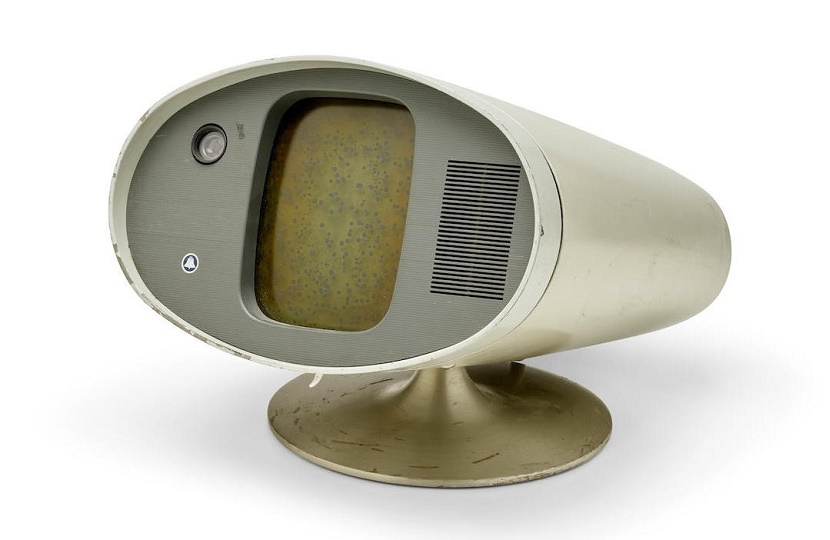
\includegraphics[width=6.99cm]{figures/picturephone.jpg}
    \caption{Primul model de Picturephone, care a fost instalat în cabine în 3 orașe din Statele Unite}
\end{figure}
\indent \par Însă primul prototip funcțional a fost demonstrat public în 7 aprilie 1927 într-o aulă din New York. Herbert Hoover, pe atunci secretarul comerțului al Statelor Unite, a apărut pe ecran din Washington D.C., fiind observat de către oficialii companiei AT\&T \cite{Videophone1927}. Apelul era unidirecțional pentru imagine și bidirecțional pentru sunet, datorită liniilor telefonice deja existente. Mai târziu, la Expoziția Mondială de la New York din 1964, AT\&T a prezentat primul Picturephone, la care publicul putea să efectueze apeluri bidirecționale către o cabină telefonică similară montată la Disneyland, folosind conexiune VHF sau UHF prin cablu \cite{Avoira2020}. Acesta a fost indisponibil pentru uz casnic până în 1970, când aceeași companie a lansat un Picturephone îmbunătațit, disponibil printr-un serviciu lunar. Din cauza costului ridicat de 160 de dolari pe lună (echivalent a 1000 de dolari în 2020), nu a prezentat interes, serviciul fiind desființat în 1973 \cite{Videophone1927}.

\section{Era digitală și tranziția către Internet}
\label{sec:ch2sec2}

\indent \par În anii '80, diverse companii, printre care Mitsubishi, au comercializat diverse videotelefoane care puteau transmite imagini statice prin intermediul rețelei telefonice deja existente, fapt care permitea folosirea modemurilor existente cu rate de transfer între 2,4 și 9,6 kilobiți pe secundă. Evoluția algoritmilor digitali de compresie a imaginilor și a lățimii de bandă, a permis ca AT\&T să mai încerce o dată cu VideoPhone 2500, care, de asemenea, nu a avut succes, costând inițial 1500 de dolari în 1992 \cite{Borth98}.
\indent \par Apariția protocoalelor Internet și a tehnicilor și mai avansate de compresie audio-video a permis ca imaginea și sunetul să fie transmise în pachete mult mai mici, rezultând în costuri mult mai reduse. Simultan cu dezvoltarea rețelei ARPANET (precursoarea Internetului), destinată inițial pentru transfer de date, s-a discutat problema comunicării în timp real prin voce \cite{RFC741}. Așadar, s-a propus în decembrie 1973 implementarea Network Voice Protocol (NVP), care a venit cu următoarele considerente: separarea semnalelor de control de traficul de date, evitarea retransmiterii pachetelor pierdute, adaptabilitate la condițiile variabile ale rețelei, precum și independența gestionării resurselor de către fiecare sistem, dar și de către protocoalele de nivel mai jos\cite{RFC741}.
\indent \par PictureTel a jucat un rol important în evoluția comunicațiilor video. Cei doi fondatori ai săi, Brian L. Hinman și Jeffrey G. Bernstein, absolvenți ai MIT și buni prieteni, au fondat PicTel în 1984 (a fost ulterior redenumită pentru a evita confuzia cu termenul \textit{pixel}) cu sprijin financiar din partea lui Robert Sterling. În 1986, după ce compania a devenit publică, a dezvoltat algoritmul Motion Compensated Transform (MCT), care a permis reducerea unei transmisii audio-video de calitate de la 768 Kb/s la 224. Pe baza acestui algoritm, au lansat codecul C-2000 în luna iulie al aceluiași an, cu ajutorul căruia PictureTel a devenit lider în domeniul său. În 1988, un nou algoritm de compresie video a fost lansat, Hierarchical Vector Quantizing (HVQ), folosit în codecul C-3000, precum și în sistemul V-2100 \cite{Root2000}. Cu ajutorul acestuia, lățimea de bandă folosită a fost redusă la jumătate, comparativ cu algoritmul MCT. În anii '90, a colaborat la crearea standardului H.320 pentru videoconferințe prin rețeaua ISDN, precum și a standardului H.323 pentru comunicare audio-video prin Internet pe baza protocolullui TCP, cel din urmă folosit pentru a crea produsul software LiveLan \cite{Root2000}.
\indent \par O dată cu migrarea videoconferințelor către Internet, au început să apară soluții gratuite, potrivite și consumatorilor de rând, care să nu ceară echipament auxiliar, pe lângă un computer și o cameră web. Una din primele aplicații influente de acest fel este realizată de Tim Dorcey la Universitatea Cornell și se numește CU-SeeMe, apărut prima dată în 1992 pentru sistemele Macintosh \ref{CUSeeMeMac}. Apelurile cu doi participanți pot fi inițiate de către unul din ei conectându-se direct la celălalt, în timp ce apelurile cu mai mulți participanți necesită conectarea fiecăruia la un \textit{reflector} CU-SeeMe \cite{Dorcey95}. \textit{Reflectorul} este un software destinat sistemelor UNIX ce are menirea de a a redistribui fluxurile de pachete, principala sa motivație fiind lipsa abilităților de multicast pe Macintosh de la vremea respectivă \cite{Dorcey95}. Pentru transmisie, imaginea se împarte în pătrate de dimensiune 8x8, acestea fiind selectate pentru trimitere doar în cazul în care gradul de similitudine este suficient de ridicat \cite{Dorcey95}. Acest grad este calculat ca sumă a tuturor diferențelor absolute între fiecare pixel de pe aceeași poziție, la care se aplică o penalizare multiplicativă pentru diferențele între pixelii apropiați \cite{Dorcey95}. Mai târziu, a adoptat standardul H.323, care s-a regăsit și pe alte produse, precum Microsoft NetMeeting (începând cu versiunea 2) \cite{Vidconf, Perey2000}.
\begin{figure}[H]
    \centering
    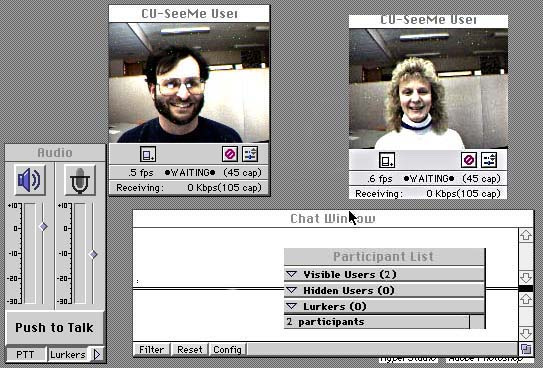
\includegraphics[width=8.8cm]{figures/cu-seeme.jpg}
    \caption{Aplicația CU-SeeMe rulând pe Macintosh}
    \label{CUSeeMeMac}
\end{figure}
\indent \par În 1994, un moment important a fost lansarea primei camere web destinate consumatorilor, Connectix QuickCam \ref{QuickCam} \cite{Wolfe2019}. Putea captura imagini doar în 16 culori la 15 cadre pe secundă și a fost inițial compatibilă doar cu Macintosh \cite{Wolfe2019}. Un an mai târziu, a fost lansată și varianta pentru Windows. Însă calitatea redusă a imaginii nu a fost un impediment pentru persoanele aflate la distanță de a se putea simți aproape una de cealaltă, de a putea interacționa, de a trăi evenimente aflate în diverse colțuri ale lumii \cite{QuickCam94}. Ulterior, au apărut variante îmbunătațite de QuickCam, cu captură de imagini color la rezoluții mai mare, dar și cu conectivitate paralelă și USB.
\begin{figure}[H]
    \centering
    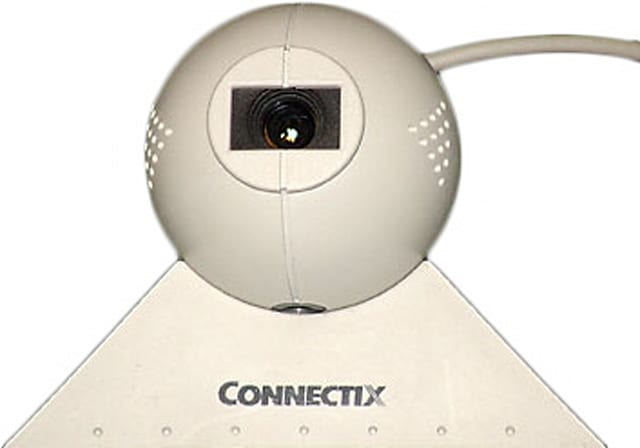
\includegraphics[width=5.7cm]{figures/quickcam.jpg}
    \caption{Connectix QuickCam, prima cameră web comercială}
    \label{QuickCam}
\end{figure}
\indent \par În paralel s-au dezvoltat o multitudine de standarde menite de a reduce și mai mult lățimea de bandă folosită, precum și de a ușura crearea de noi platforme de comunicare. În 1997 a fost creat Session Initiation Protocol (SIP), prin care utilizatori pot fi invitați la participarea într-o sesiune multimedia, sau chiar servere prin care se poate înregistra sesiunea \cite{rfc2543}. Este o combinație dintre Session Invitation Protocol și dintre Simple Conference Invitation Protocol, prin care se încearcă potrivirea lui SIP pe o infrastructură mai flexibilă care include și alte protocoale, precum SDP, HTTP și RTSP \cite{rfc2543}. Poate funcționa atât peste TCP, cât și peste UDP, pentru o performanță îmbunătațită \cite{rfc2543}.
\indent \par Codecurile video au continuat de-a lungul timpului să evolueze. În 2003, Unitatea Internațională a Telecomunicațiilor (ITU - Internation Telecommunication Union) a făcut public standardul H.264, destinat codării audio-video în aplicații precum televiziunea prin cablu și satelit, videoconferințe prin Internet, dar și filme stocate pe medii de stocare optice \cite{H.264}. Folosește tehnici precum partiționarea imaginilor în macroblocuri, precum și codificare predictivă bidirecțională. A fost dezvoltat împreună cu ISO MPEG (Moving Picture Experts Group) \cite{H.264}.
\indent \par Între timp, au apărut platforme de mesagerie instantă precum AOL Instant Messenger (AIM) în 1997, Yahoo! Messenger în 1998, MSN Messenger în 1999 \cite{Wolfe2019}. Toate au suportat apeluri video în 2003, folosind, în principiu, SIP pentru a iniția apelurile și RTP pentru transportul pachetelor. Apple a lansat în 2002 un client pentru AIM numit iChat, folosind implementarea oficială a protocolului furnizată de America Online \cite{Wolfe2019}. iChat a primit suport pentru codecul H.264 în 2004, oferind calitate mai bună decât predecesorul său, H.263 \cite{Royal2007}.
\indent \par Însă mult mai popular pentru apelurile video a devenit Skype, care, când a fost lansat în 2003 de KaZaa, permitea apeluri gratuite în grup de 25 de persoane. Promitea, la momentul respectiv, calitate a vocii superioară față de alternativele Yahoo și MSN, dar și o traversare facilă a NAT-urilor și firewall-urilor \cite{Baset2004}. Singurul rol al serverului central era doar de login, informațiile utilizatorilor fiind păstrate într-o manieră descentralizată, prin intermediul nodurilor și supernodurilor \ref{SkypeNet} \cite{Baset2004}. Un nod ce dispune de suficientă putere de procesare și lățime de bandă fi candidat pentru a fi supernod \cite{Baset2004}. Se presupunea că fiecare nod folosește o variație a protocolului STUN pentru a comunica pe rețeaua suprapusă Skype \cite{Baset2004}. De asemenea, fiecare nod își păstra o listă de supernoduri cu care să facă legătura; această listă fiind denumită \textit{host cache} și este păstrată în registrul Windows \cite{Baset2004}. Ulterior, Skype a fost cumpărat de Microsoft în 2011 și a renunțat la topologia cu supernoduri pentru o scalabilitate mai bună, folosind, în schimb, serverele Microsoft, cu toate că au existat suspiciuni privind securitatea serviciului \cite{Whittaker2013}.
\indent \par Apoi, a urmat înglobarea unei colecții de protocoale precum SDP, STUN, TURN și RTP, precum și a unor codecuri precum VP8, G.711 și iLBC într-un proiect numit WebRTC, care vine inclus cu majoritatea browserelor moderne și pe baza căruia s-au construit majoritatea aplicațiilor moderne precum Microsoft Teams, Zoom, Jitsi Meet și OBS.Ninja, care s-au dovedit esențiale în mediul profesional și academic pe parcursul epidemiei de coronavirus începută în 2019 și care continuă și în 2021.
\begin{figure}
    \centering
    \scalebox{0.75}{\input{figures/skypenetwork.pdf_tex}}
    \caption{O reprezentare a topologiei de rețea folosită de Skype}
    \label{SkypeNet}
\end{figure}